\chapter{Index Construction}
In these chapter we will analyze how we construct inverted index and storage in memory/disk, we will consider 
\emph{SPIMI} (Single-pass in-memory indexing) and \emph{Multi-way Merge-sort}, but also distributional caching.

\section{SPIMI approach}
SPIMI is an approach to storage inverted index using a single pass in memory and has two key ideas:
\begin{enumerate}
	\item Generate separate dictionaries for each block of docs (no need for term map to termID)
	\item Accumulate postings in lists as they occur in each block of docs, in internal memory.
\end{enumerate}
With this approach we generate an inverted index for each block, where also compression is possible and 
in figure \ref{img:spimi} there is the pseudocode of SPIMI approach.

\begin{figure}
	\caption{SPIMI pseudocode}
	\label{img:spimi}
	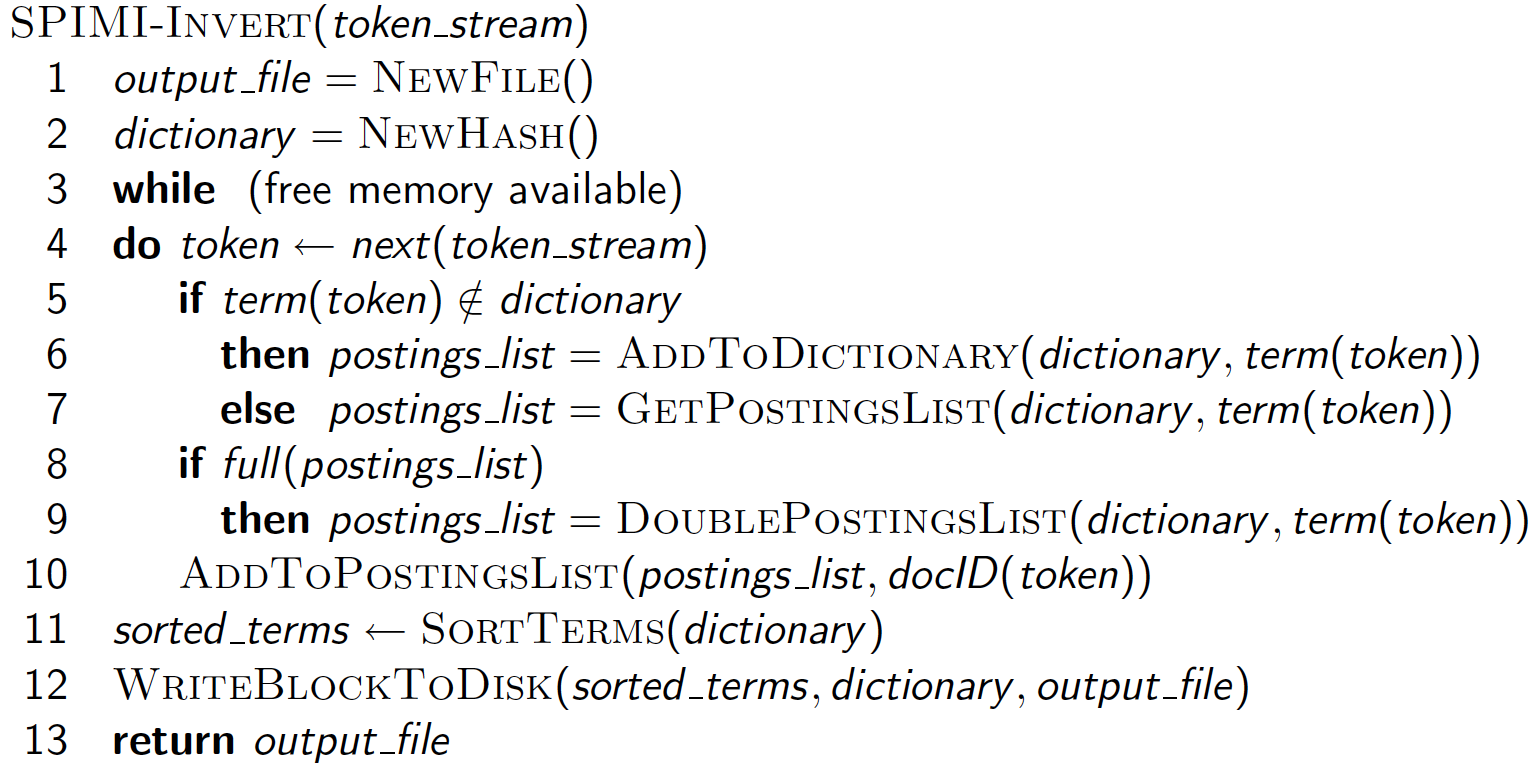
\includegraphics[width=\textwidth]{Images/spimi}
\end{figure}
There are some problems with this approach, like we decide always to double dimension of block when is full, also 
we assign TermID, create pairs $<termID, docID>$ and sort pairs by TermID.

Given a query $q$ we require $N / m$ queries whose results have to be combinated, where $N$ is the number of items 
and $m$ is the dimension of main memory.


To sort $n$ inverted index we accumulate terms, and in a certain time we will encounter again, so we 
assume $|\text{dictionary}| \leq M$ and we have the following steps:
\begin{enumerate}
    \item Scanning and build dictionary of distinct tokens.
    \item Sort the tokens, assign lexicografic IDs such that $T_1 \leq_L T_2 \To ID(T_1) \leq ID(T_2)$
    \item Scan documents and we create pair $<term ID, docID>$.
    \item Sort by first component and then to second component and since the order of terms are 
	  lexicografically sort of first component is this correct.
    \item Decode termID, such that scanning pair in substituting termID with terms, by using the internal
	  memory dictionary.
\end{enumerate}
This sorting is stable, a properties that means that we keep reciprocal order of equal items.

\section{Multi-way merge sort}
We will now consider the multi-way merge-sort, called also \emph{BSBI} (Blocked sort-based Indexing), that consist that
we map term to termID to be kept in memory for construction the pairs and needs two passes, unless we use hashing
and thus with some probability of collision.

This merge-sort consist in particular in two phases:
\begin{enumerate}
    \item Scan input and divide on block of size $M$, where we have for each block $2M/B$ I/Os where $B$ 
	  is the size of block.\newline
	  The total cost of this step is $\frac{2M}{B} * \frac{n}{M} = O(\frac{n}{B})$ I/Os.
    \item Merge $X = M/B-1$ runs, given a $\log_X N/M$ passes, as we can see in figure \ref{img:multiWayMerging}

	  \begin{figure}
	      \caption{Multiway Merge-sort merging}
	      \label{img:multiWayMerging}
	      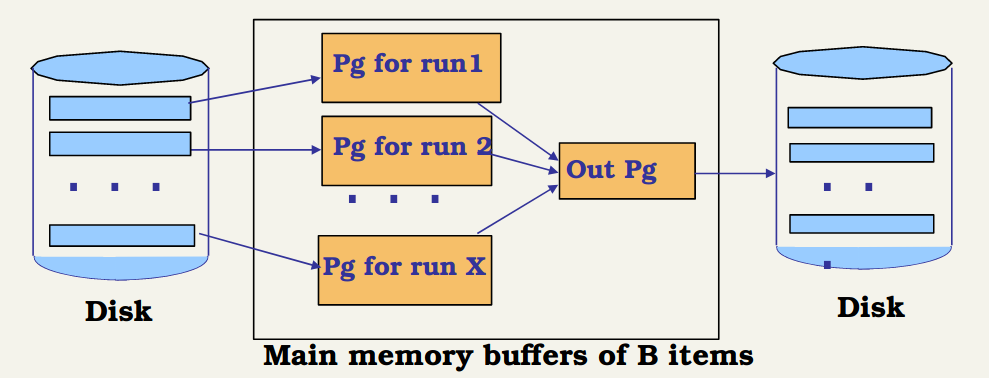
\includegraphics[width=\textwidth]{Images/multiwayMerge}
	  \end{figure}
	  We have to compare $k$ minimum comparison to find the smallest and write in output and in case 
	  output is full we have to flush on memory harddisk/SSD, so we have $O(\frac{X}{B})$ I/Os to find
	  a list of $X$ items in $k$ sorted rows, and we have $\log _k \frac{n}{M}$ levels,
	  yields to a total cost of $O(\frac{n}{B} \log_k \frac{n}{M})$.
\end{enumerate}

\section{Distributed indexing}
For web-scale indexing we must use a distributing computing cluster of inverted index, and since $2004$
Google use \emph{Map Reduce}, that we will introduce later, but we now introduce the distributed indexing.

We maintain a master machine directing the indexing job, considered “safe” and we break up indexing 
into sets of (parallel) tasks, where master machine assigns tasks to idle machines and other machines
can play many roles during the computation.\newline
We will use two sets of parallel tasks, Parsers and Inverters, so we break the document collection in two ways:
\begin{description}
	\item [Term-based partition: ] one machine handles a subrange of terms,
		                       as we can note in figure \ref{img:termBased}.
    \item [Doc-based partition: ] one machine handles a subrange of documents, 
	    			  as we can note in figure \ref{img:docBased}.
\end{description}

\begin{figure}
	\caption{Term-based Distributed indexing}
	\label{img:termBased}
	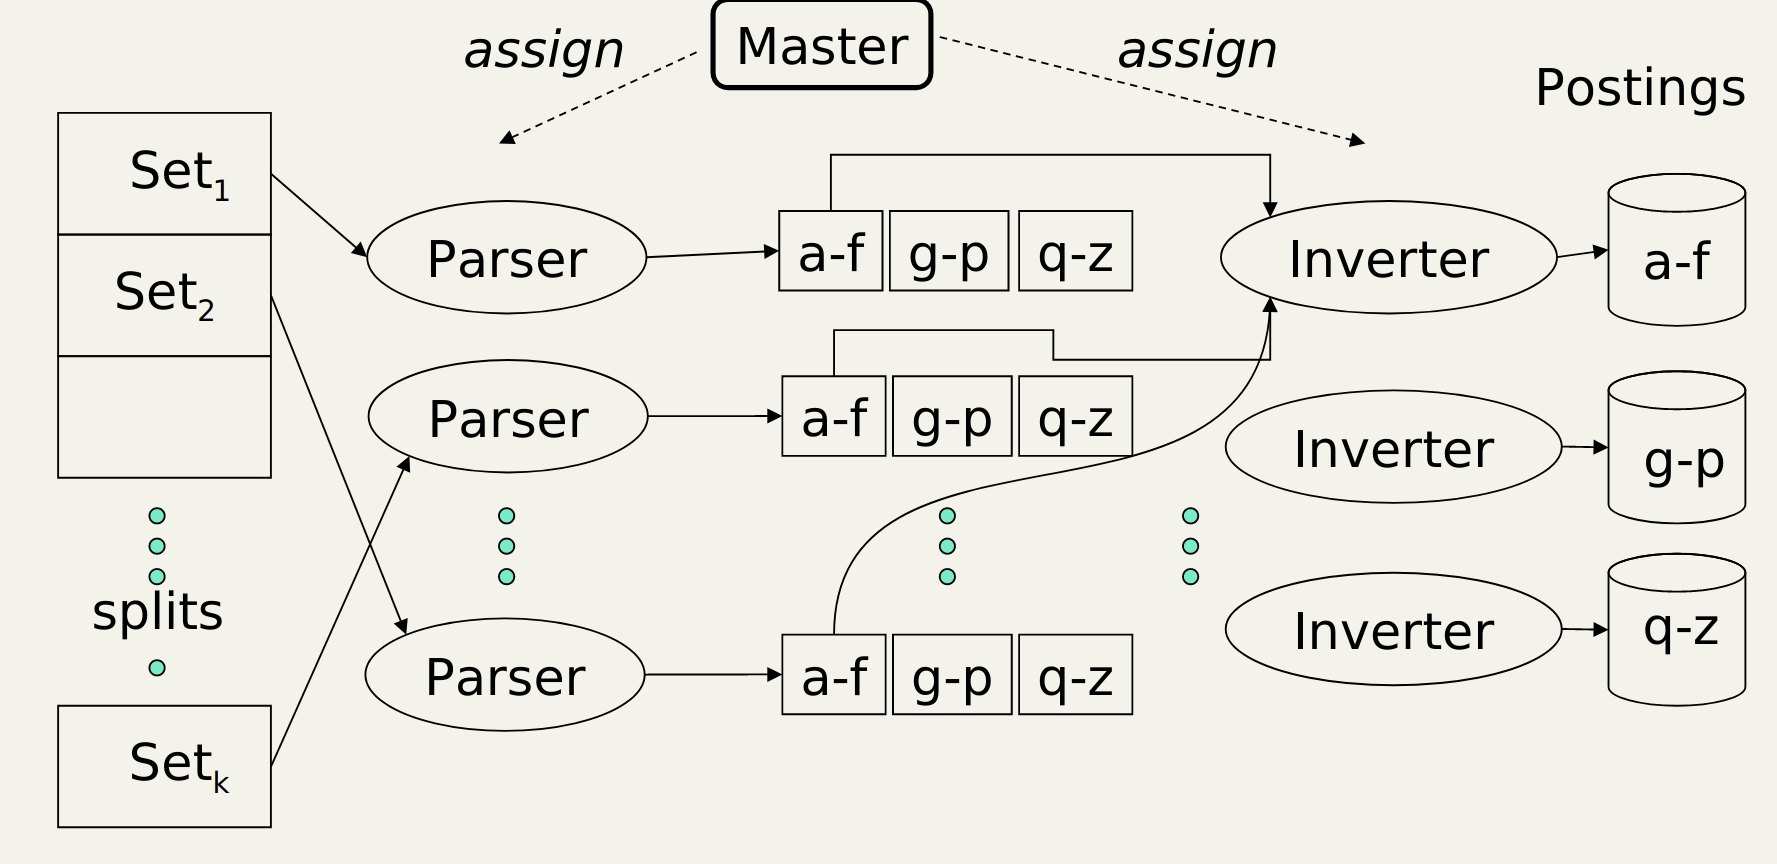
\includegraphics[width=\textwidth]{Images/termBased}
\end{figure}
\begin{figure}
	\caption{Doc-based Distributed indexing}
	\label{img:docBased}
	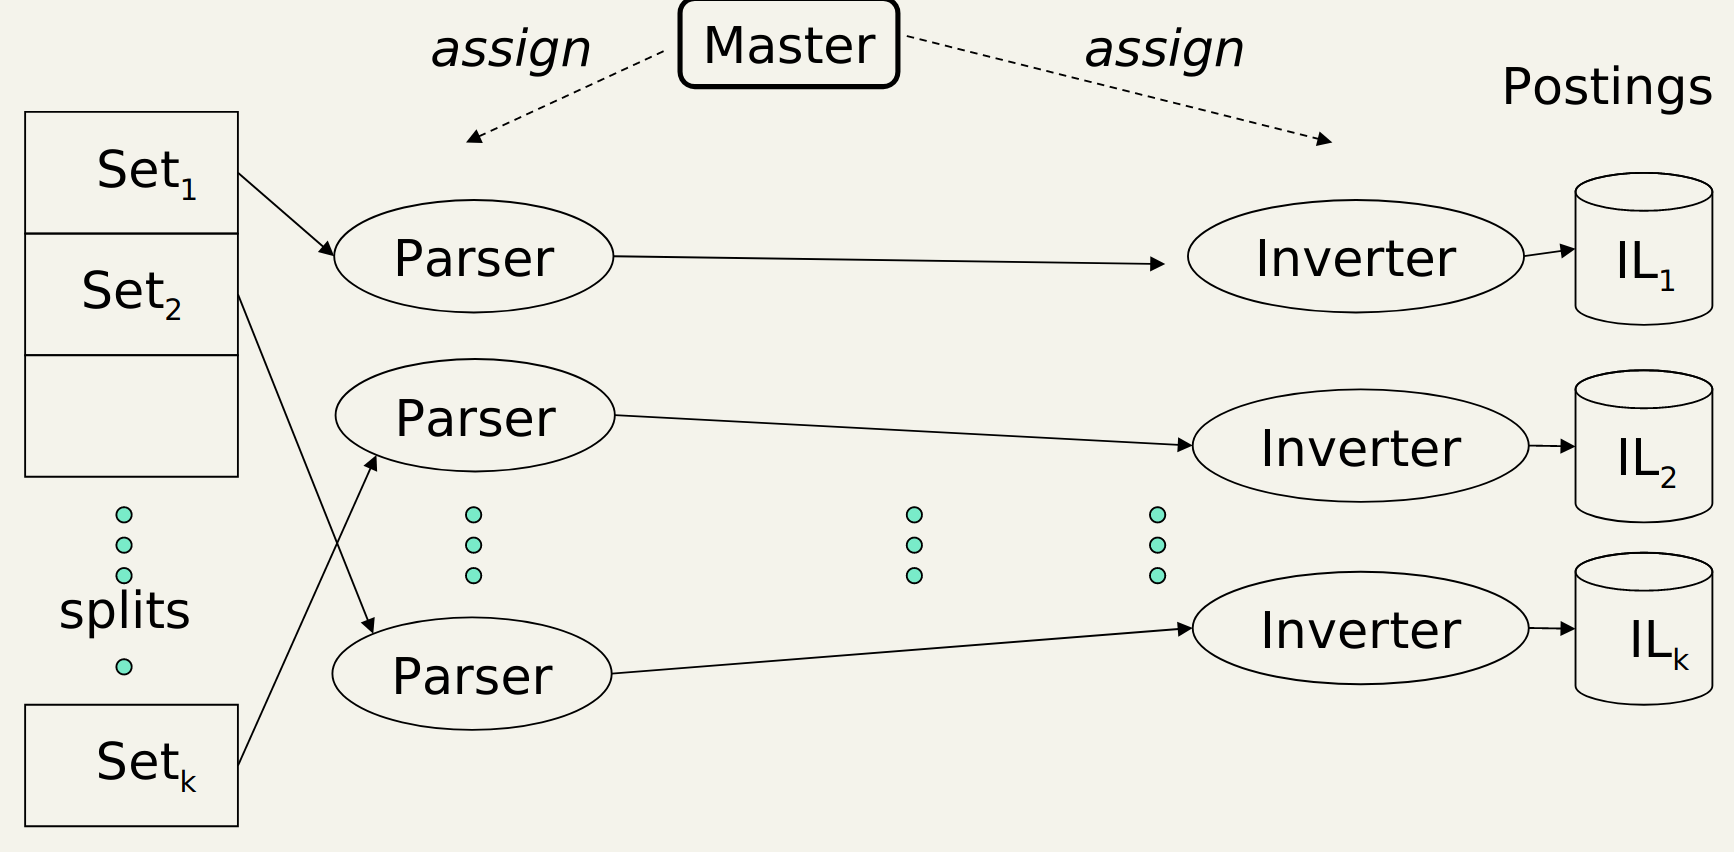
\includegraphics[width=\textwidth]{Images/docBased}
\end{figure}
\emph{MapReduce} is a robust and conceptually simple framework for distributed computing, 
without having to write code for the distribution part and Google indexing system (ca. $2004$) 
consists of a number of phases, each implemented in MapReduce.

Up to now, we have assumed static collections, now more frequently occurs that documents come in over time
and documents are deleted and modified, so this induces postings updates for terms already in dictionary
and new terms added/deleted to/from dictionary.

A first approach is to maintain “big” main index, and new docs go into “small” auxiliary index, where 
we search across both, and merge the results.\newline
In case of deletions we use an invalidation bit-vector for deleted docs, so we filter search results
by the invalidation bit-vector and periodically, we re-index into one main index.

The problem is this approach is that has poor performance: merging of the auxiliary index into the main index
is efficient if we keep a separate file for each postings list and merge is the same as a simple append
[new docIDs are greater] but this needs a lot of files so is inefficient for O/S, anyway
in reality we use a scheme somewhere in between, like split very large postings lists, 
collect postings lists of length $1$ in one file and so on.

We introduce now \emph{Logarithmic merge}, where we maintain a series of indexes, 
each twice as large as the previous one ($M, 2M , 2^2 M, 2^3 M, \dots 2^iM$) and we keep a small index
$Z$ in memory of size $M$ and we store $I_0, I_1, I_2, \dots$ on disk and if $Z$ gets full, 
we write to disk as $I_0$ or merge with $I_0$ (if I0 already exists).\newline
Either write $Z + I0$ to disk as $I_1$ (if no I1) or merge with $I_1$ to form $I_2$, and so on.

Some analysis, with $C = $total collection size) we have that auxiliary and main index has that 
each text participates to at most $(C/M)$ mergings because we have $1$ merge of the two indexes (small and large)
every $M$-size document insertions, instead in logarithmic merge each text participates to no more than
$\log (C/M)$ mergings because at each merge the text moves to a next index and they are at most $\log (C/M)$.

Most search engines now support dynamic indexing (news items, blogs, new topical web pages), 
but (sometimes/typically) they also periodically reconstruct the index, query processing is then
switched to the new index, and the old index is then deleted.

